
%%%%%%%%%%%%%%%%%%%%%%%%%%%%%%%%%%%%%%%%%
% Beamer Presentation
% LaTeX Template
% Version 1.0 (10/11/12)
%
% This template has been downloaded from:
% http://www.LaTeXTemplates.com
%
% License:
% CC BY-NC-SA 3.0 (http://creativecommons.org/licenses/by-nc-sa/3.0/)
%
%%%%%%%%%%%%%%%%%%%%%%%%%%%%%%%%%%%%%%%%%

%----------------------------------------------------------------------------------------
%	PACKAGES AND THEMES
%----------------------------------------------------------------------------------------

\documentclass{beamer}

\mode<presentation> {

% The Beamer class comes with a number of default slide themes
% which change the colors and layouts of slides. Below this is a list
% of all the themes, uncomment each in turn to see what they look like.

%\usetheme{default}
%\usetheme{AnnArbor}
%\usetheme{Antibes}
%\usetheme{Bergen}
%\usetheme{Berkeley}
%\usetheme{Berlin}
%\usetheme{Boadilla}
%\usetheme{CambridgeUS}
%\usetheme{Copenhagen}
%\usetheme{Darmstadt} %Nice
%\usetheme{Dresden} %Nice
\usetheme{Frankfurt} %Nice
%\usetheme{Goettingen} %Sidebar
%\usetheme{Hannover}
%\usetheme{Ilmenau}
%\usetheme{JuanLesPins}
%\usetheme{Luebeck}
%\usetheme{Madrid}
%\usetheme{Malmoe}
%\usetheme{Marburg}
%\usetheme{Montpellier}
%\usetheme{PaloAlto}
%\usetheme{Pittsburgh}
%\usetheme{Rochester}
%\usetheme{Singapore}
%\usetheme{Szeged}
%\usetheme{Warsaw}

% As well as themes, the Beamer class has a number of color themes
% for any slide theme. Uncomment each of these in turn to see how it
% changes the colors of your current slide theme.

%\usecolortheme{albatross}
%\usecolortheme{beaver}
%\usecolortheme{beetle}
%\usecolortheme{crane}
%\usecolortheme{dolphin}
%\usecolortheme{dove}
%\usecolortheme{fly}
%\usecolortheme{lily}
%\usecolortheme{orchid}
%\usecolortheme{rose}
%\usecolortheme{seagull}
%\usecolortheme{seahorse}
%\usecolortheme{whale}
%\usecolortheme{wolverine}

%\setbeamertemplate{footline} % To remove the footer line in all slides uncomment this line
%\setbeamertemplate{footline}[page number] % To replace the footer line in all slides with a simple slide count uncomment this line

%\setbeamertemplate{navigation symbols}{} % To remove the navigation symbols from the bottom of all slides uncomment this line
}

%%% SYMBOLS AND STYLES %%%

\DeclareSymbolFont{symbolsC}{U}{txsyc}{m}{n} 
\DeclareMathSymbol{\strictif}{\mathrel}{symbolsC}{74}
\usepackage{multicol}
\newcommand{\tuple}[1]{\langle#1\rangle} %%Angle brackets
\setbeamercovered{transparent}
\usepackage{graphicx}

	
%%% CITATIONS %%%
\usepackage[round]{natbib} %%Or change 'round' to 'square' for square backers
\setcitestyle{aysep={}}
\newcommand\citeapl[2][]{\citeauthor{#2}'s#1} %%Use \citeapl is for possessive author name only.
\newcommand\citea[2][]{\citeauthor{#2}#1} %%Use \citea is for author name only, with optional page numbers.
\newcommand\citepl[2][]{\citeauthor{#2}'s (\citeyear[#1]{#2})}%%The command \citepl is for possessive citations.
\usepackage{bibentry}

\usepackage{graphicx} % Allows including images
\usepackage{booktabs} % Allows the use of \toprule, \midrule and \bottomrule in tables

%----------------------------------------------------------------------------------------
%	TITLE PAGE
%----------------------------------------------------------------------------------------

\title[Short title]{IEEE\_student\_contest\_2021} % The short title appears at the bottom of every slide, the full title is only on the title p wage

\author{Cem Gülşan and Valentin Resapow} % Your name
\institute[Institute of Electromagnetic Theory] % Your institution as it will appear on the bottom of every slide w, may be shorthand to save space
{
Institute of Electromagnetic Theory\\ % Your institution for the title page
\medskip
\textit{cem.guelsan@tuhh.de}\\ % Your email address
\textit{valentin.resapow@tuhh.de}
}
\date{\today} % Date, can be changed to a custom date

\begin{document}

\begin{frame}
\titlepage % Print the title page as the first slide
\end{frame}

\begin{frame}
\frametitle{List of contents}

\tableofcontents[hideallsubsections]

\end{frame}

%----------------------------------------------------------------------------------------
%	PRESENTATION SLIDES
%----------------------------------------------------------------------------------------

%%% NOTES %%%

%Recall: \pause for 

%Recall: ITEMIZE

%\begin{itemize}  
%\item<1-> 
%\end{itemize}

%\onslide<1->{ SLIDE }

%\begin{itemize}[<+(1)->]
%\begin{itemize}[<+->]

%------------------------------------------------
\section{task definition} 
%------------------------------------------------

% \subsection{FIRST SUB}

\begin{frame}
\frametitle{task definition}

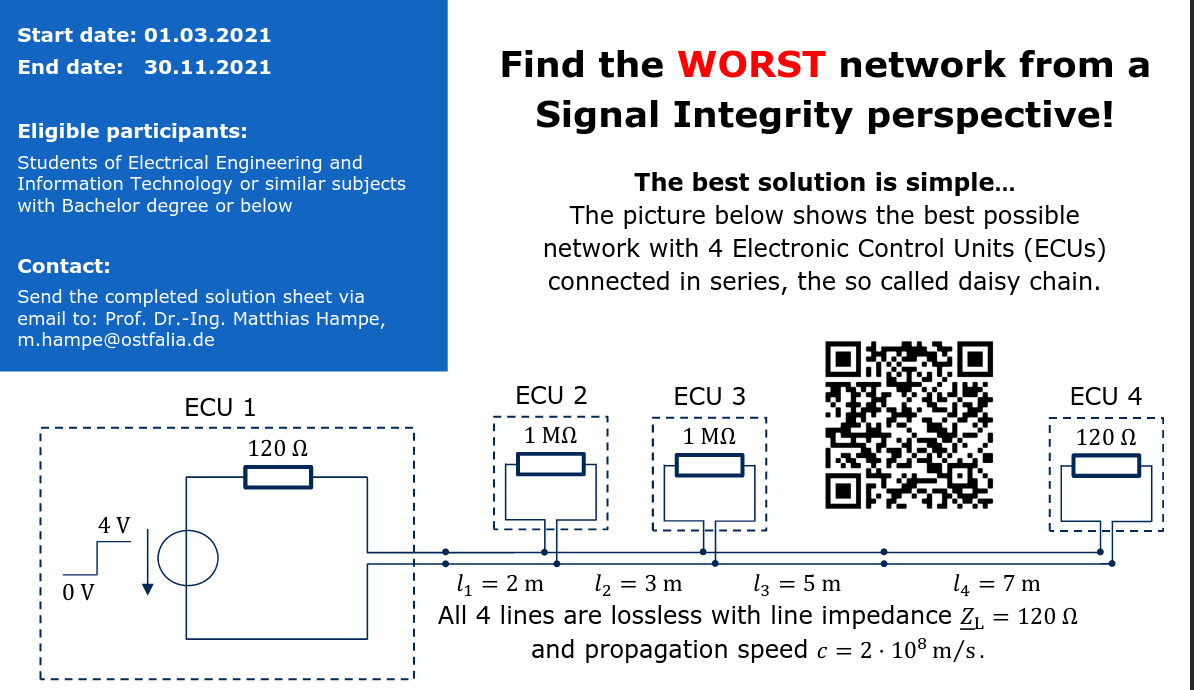
\includegraphics[width=12cm, height=7cm]{task_defintion.png}
\end{frame}


%------------------------------------------------
\section{first approach} 
%------------------------------------------------

\begin{frame}
\frametitle{analytical approach}
TODO: Zeichung in Inkscape von unsere besten analytischen Lösung
\begin{itemize}
    \item CFK
    \item OSB
    \item Siebdruckplatte
\end{itemize}
\end{frame}


%------------------------------------------------
\section{section approach} 
%------------------------------------------------
\begin{frame}
\frametitle{brute force approach}
TODO: Zeichung in Inkscape von
\begin{itemize}
    \item CFK
    \item OSB
    \item Siebdruckplatte
\end{itemize}
\end{frame}
%----------------------------------------------------------------------------------------
\begin{frame}
\frametitle{some statistics}
TODO: Git Zeugs suchen 

\begin{itemize}
    \item CFK
    \item OSB
    \item Siebdruckplatte
\end{itemize}
\end{frame}
\nobibliography{Zotero}
\bibliographystyle{PhilReview}
\nobibliography{Zotero}

\end{document} 
